\subsection{Introduction}
Neural signals are firstly recorded as raw data. They exhibit two
main components:
\begin{itemize}
    \item Local field potentials (LFPs) exist at low frequencies (0.1-300 Hz).
    \begin{figure}[H]
        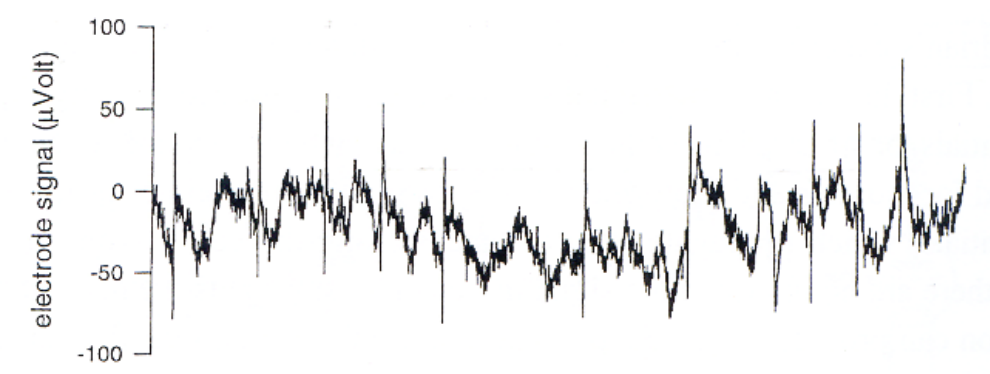
\includegraphics[scale=0.45]{2_1}
        \centering
    \end{figure}
    \item Spikes (MUA) exist at higher frequencies (300-3000 Hz).
    \begin{figure}[H]
        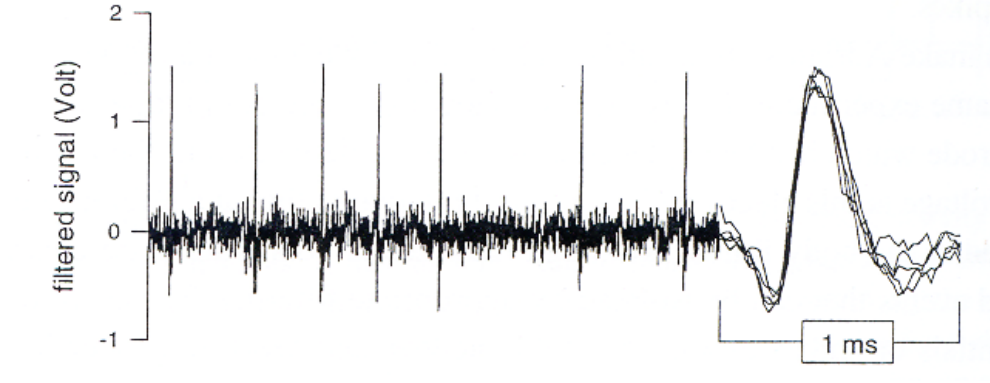
\includegraphics[scale=0.45]{2_2}
        \centering
    \end{figure}
\end{itemize}
The signal is obtained through extracellular recordings,
then amplified and filtered. There are 3 possible situations, according to the
distance of the electrode tip from the neurons:
\begin{itemize}
    \item \(<50\,\mu{m}\): the SNR is good enough to distinguish the activity
    of a single neuron (single unit).
    \item \(50\sim150\,\mu{m}\): spikes are still detected, but the difference in
    their shape is masked by the noise (multi-unit activity or MUA).
    \item \(>150\,\mu{m}\): spikes cannot be detected and they contribute to
    the noise.
\end{itemize}
\begin{figure}[H]
    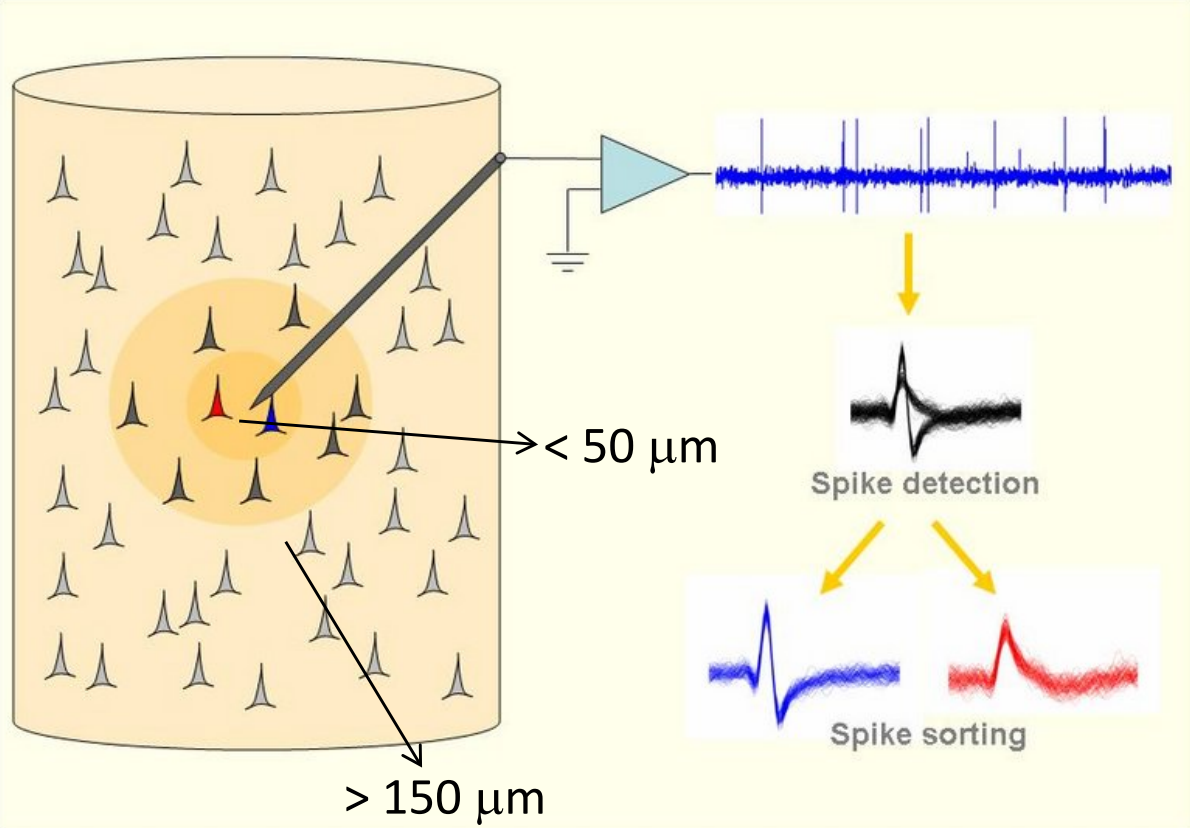
\includegraphics[scale=0.35]{2_3}
    \centering
\end{figure}
\newpage
When recording data from 1 electrode, there are two patterns of activity:
\begin{itemize}
    \item Spike: single over-threshold signal representing the electrical
    activity of one or more neurons.
    \item Burst: sequence of highly packed spikes often occurring simultaneously
    on several channels and giving rise to a phenomenon known as
    'network burst'.
\end{itemize}
In the following it is show the Data Preprocessing workflow:
\begin{figure}[H]
    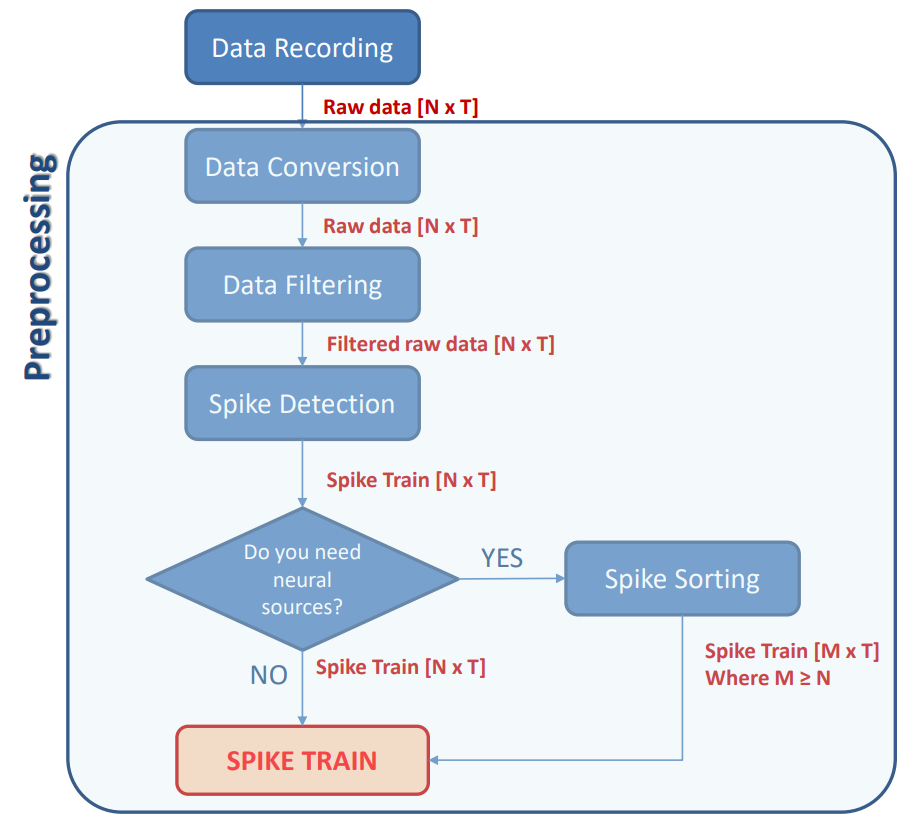
\includegraphics[scale=0.6]{2_4}
    \centering
\end{figure}
Spike trains are defined as the temporal sequence of spiking events, without
any regard of time. Spike trains are mathematically defined as follow:
\begin{itemize}
    \item Single channel spike train: \(ST(t)=\sum_{s=1}^{N}\delta{(t-t_s)}\)
    \item Multiple channel spike train: \(ST_j(t)=\sum_{s=1}^{N_j}\delta{t-t_s}\)
    with \(j=1,...,M\)
\end{itemize}
\begin{figure}[H]
    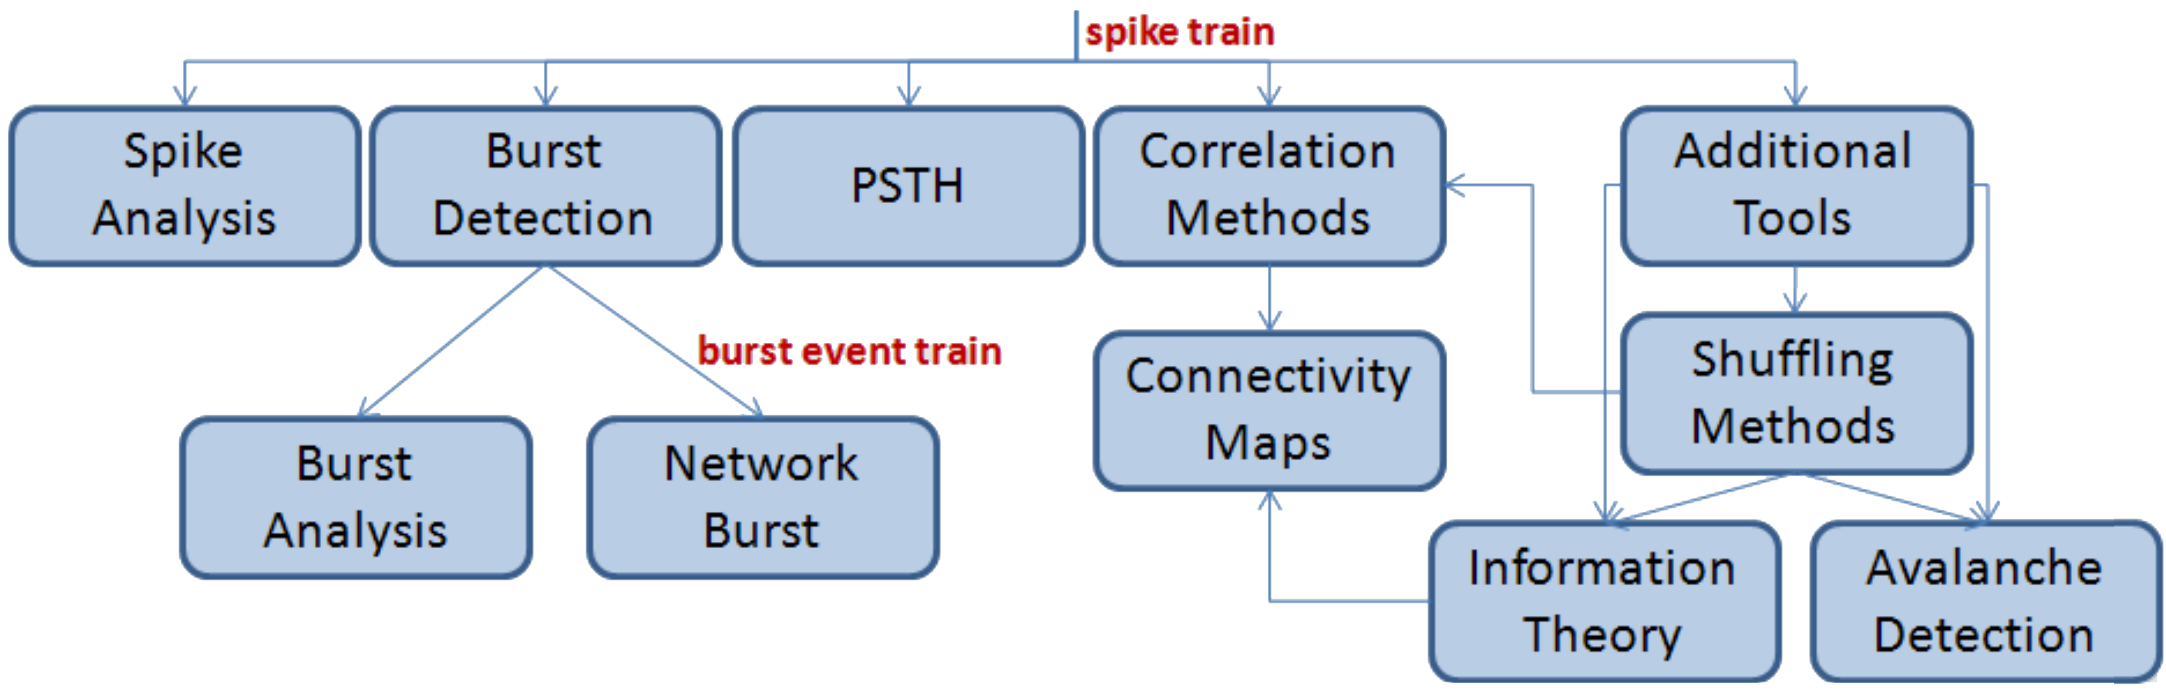
\includegraphics[scale=0.45]{2_5}
    \centering
\end{figure}
\textbf{Spike Detection:} it consists in recognizing the spikes within the raw data.\\
It is the most important step of the analysis, as it affects all
the subsequent steps.\\
\textbf{Spike Sorting:} associate each spike to a specific putative source
(classify spikes).\\
When performing Spike Detection there are two main issues:
\begin{itemize}
    \item Reliability (of the selected detection method)
    \item Precise position (of the detected peaks in the spike train)
\end{itemize}


\subsection{Spike Detection algorithms}
Therefore, several algorithms (each one with pros and cons) have been developed.
These spike detection algorithms can be divided into 3 families:
\begin{itemize}
    \item Thresholding: it is assumed that spikes peak-to-peak amplitude is larger
    than the noise level.
    \item Energy operator: non-linear energy operator accentuating high frequency
    contet, i.e. spikes.
    \item Template matching: it is an approach based on the spike shape,
    involving Spike Sorting.
\end{itemize}
\subsubsection{Thresholding algorithms}
\paragraph{Simple Hard Threshold}
A threshold value is defined (either positive or negative). If the signal
overcomes the threshold, then a spike is detected. A refractory period (RP)
is employed to account for subsequent samples overcoming the threshold after
a spike detection.
\paragraph{Hard Threshold} Notice this algorithm is applied also to
absolute-valued signals. It involves 2 distinct main steps:
\begin{itemize}
    \item Application of a threshold
    \item Spike identification
\end{itemize}
A time window denoted by \(T\) is applied to the signal, centering the window
\(\frac{1}{3}T\) before the detected spike. The length of \(T\) is to be
carefully chosen, usually \(1-3\,ms\), as it must minimize the likelihood that
more than one spike is captured in the window.\\
The threshold (\(Thr\)) is defined in several ways:
\begin{itemize}
    \item \(Thr=n\sigma[V]\): \(n\) times the standard deviation (SD) of
    the noise.
    \item \(Thr=aP2P[V]\): fraction of the full amplitude (peak-to-peak) of
    the signal.
    \item \(Thr=n\sigma_N[V]\): \(n\) times the SD estimated from the Median
    Absolute Deviation (\(MAD\)), with \(MAD=median(|x-median(x)|)\).
\end{itemize}
\paragraph{Hard Threshold Local Maxima}
This method is very similar to the previous ones, but the spike position is
associated to the local maxima (and not set at the time of the first sample
overcoming the threshold).
\paragraph{Hard Threshold Differential Threshold}
A sliding window \(W\) is sized to contain at least one spike and is shifted
over the signal. The peak-to-peak threshold \(k\sigma\) is a multiple of the
noise standard deviation. Then, a spike is detected in the \(i-\)th window
when \([(max_i-min_i)\ge{k\sigma}]\), with \(i=1,...,\frac{T}{W}\) and \(T\)
being the signal whole duration.\\
This approach exhibit a major issue: undersampling if more spikes are found in
a single window (typically at the window borders).
\paragraph{Precision Timing Spike Detection (PTSD)}
This method solves the undersampling issue. The max and min of each selected
window is selected. A refractory period RP is also considered. This technique
is more demanding from the computational point of view, but it allows to detect
also the spikes passing through the boundaries of the considered bin.
\subsubsection{Energy operator algorithms}
\paragraph{Signed Energy (SE)}
A moving window is used to scan the signal. For each time window the energy is
computed as follow:
\begin{align*}
    SE(i)=\frac{1}{W}\sum_{j=i-\frac{W}{2}}^{j+\frac{W}{2}}V(j)^2
\end{align*}
where V are the voltage amplitudes within the window and W is the window width.
The result is multiplied by +1 when the average amplitude of the raw signal is
positive, -1 when negative.
\paragraph{Nonlinear Energy Operator (NEO)}
The NEO is defined such that:
\begin{itemize}
    \item Constant voltage or zero \(\Rightarrow NE=0\)
    \item Waveform rapidly varying and a large amplitude
    \(\Rightarrow NE \text{ is maximum}\).
\end{itemize}
The \(NE\) of a signal \(x(n)\) is defined as:
\begin{align*}
    \psi[x(n)]=x^2(n)-x(n+1)\cdot x(n-1)
\end{align*}
Notice that the NEO is defined for each sample \(i\) and computed within a
window \(W\) centered in \(i\).\\
As a consequence, the NEO is large only when the signal \(x(n)\) is high is both
power and frequency. This method works especially well as a spike is generally
characterized by localized high frequencies and an increase in instantaneous
energy.\\
The threshold is defined as a scaled mean of the NEO:
\begin{align*}
    Thr=C\frac{1}{N}\sum_{n=1}^{N}\psi[x(n)]
\end{align*}
\subsection{Performance evaluation}
In order to assess the performance of a Spike Detection algorithm, a groundtruth
is to be defined, such that several metrics of the tested algorithm can be
computed. A groundtruth is a collection of information (typically a dataset)
which is known to be true, opposed to information provided by inference.
There are 3 main types of groundtruths:
\begin{itemize}
    \item Experimental groundtruth: neurons are recorded into two distinct ways,
    extracellular and intra-cellular (or juxtacellular), then a researcher uses
    the precise intra-cellular recordings (exhbiting precise timing and
    localization) to find the same spikes into the extracellular signal.
    \item Computational groundtruth: data are synthetic and produced by a
    model reproducing the behaviour of a network of neurons under different
    conditions. In particular, this method enables the researcher to test the
    Spike Detection algorithms against dataset with different characteristics,
    such as different signal-to-noise ratios (SNR).
    \item Hybrid groundtruth: natural and synthetic data can be mixed as well. In
    particular, it is common to exploit manually detected and sorted spikes to be
    fed into computational models as input.
\end{itemize}
Several distinct metrics might be taken into account when evaluating the
performance of Spike Detection algorithm, in particular the most used ones are:
\begin{itemize}
    \item Error count:
    \begin{itemize}
        \item Type I error \(\Rightarrow\) False Positive (FP): incorrect
        inclusion of noise, or spikes or other cells.
        \item Type II error \(\Rightarrow\) False Negative (FN): omission of
        true spikes.
    \end{itemize}
    \item Evaluation of the position of the detected spike (mean error)
    \item ROC curve
\end{itemize}
Let's define the following variables:
\begin{itemize}
    \item \(NREF\): number of reference spikes (true spikes present in
    the groundtruth dataset)
    \item \(NDS\): number of detected spikes (spikes identified by the
    tested Spike Detection algorithm)
    \item \(NCS\): number of correspondent spikes (spikes correctly
    identified by the algorithm matching the groundtruth data)
\end{itemize}
At this point, the following expressions for False Positives and False Negatives
can be derived:
\begin{align*}
    \text{False Positives}\Rightarrow FP=NDS-NCS
    \quad\quad\quad
    \text{False Negatives}\Rightarrow FN=NREF-NCS
\end{align*}
\begin{figure}[H]
    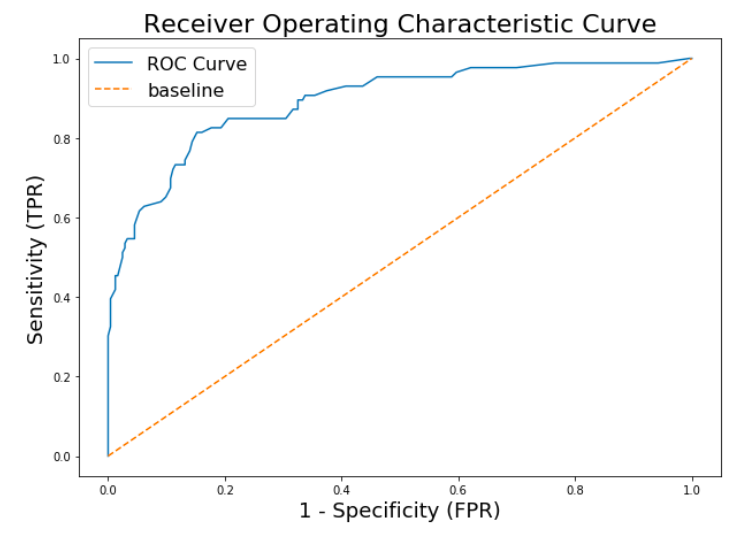
\includegraphics[scale=0.4]{2_6}
    \centering
\end{figure}
Another way to rapidly visualize and assess the performance are the Receiver
Operating Characteristic (ROC) curve and the Area Under the Curve (AUC), reducing
the curve to a single scalar value between 0 and 1. Notice that the ROC curve
provides information regarding False Positives, but nothing is said about
False Negatives.\\
Let's also list the following metrics:
\begin{align*}
    \begin{matrix}
        TP_{rate} && \frac{TP}{P}\\
        FP_{rate} && \frac{FP}{N}=1-specificity\\
        Sensitivity && \frac{TP}{TP+FN}=\frac{TP}{P}=TP_{rate}\\
        Specificity && \frac{TN}{TN+FP}=\frac{TN}{N}\\
        Accuracy && \frac{TP+TN}{P+N}\\
        Performance && \frac{TP}{FP+FN}\\
        Efficiency && \frac{Performance}{Performance+1}
    \end{matrix}
\end{align*}